\subsection{Các Vấn Đề Nâng Cao}


\subsubsection{Đa Cộng Tuyến và Hệ Số VIF}

Đa cộng tuyến xảy ra khi các cột của $\mathbf{X}$ có tương quan cao,
khiến $\mathbf{X}^T\mathbf{X}$ gần suy biến. Hệ quả là ước lượng
$\hat{\boldsymbol{\beta}}$ không ổn định, phương sai lớn dù $R^2$ cao.

\begin{tcolorbox}[mycodebox, colback=blue!3!white, colframe=blue!40!black,
    title={\textbf{Định nghĩa 1.4} - Variance Inflation Factor (VIF)}]
\begin{equation}
    \mathrm{VIF}_j = \frac{1}{1 - R_j^2},
    \label{eq:vif}
\end{equation}
trong đó $R_j^2$ là hệ số xác định khi hồi quy biến $X_j$ theo tất cả
các biến còn lại. Quy tắc thực hành: $\mathrm{VIF}_j > 10$ cho thấy
đa cộng tuyến nghiêm trọng.
\end{tcolorbox}

\textbf{Cài đặt Python - F5: \texttt{vif}}:

\begin{lstlisting}[language=Python, caption={Hàm \texttt{vif} - tính VIF cho từng biến, dùng F1 và F3}]
def vif(X: list[list[float]]) -> list[float]:
    """F5: Tinh VIF_j = 1 / (1 - R_j^2) cho moi bien j."""
    p = len(X[0])
    vif_list = []
    for j in range(p):
        # Bien phu thuoc: cot j; bien doc lap: cac cot con lai
        y_j = [X[i][j] for i in range(len(X))]
        X_j = [[X[i][k] for k in range(p) if k != j]
               for i in range(len(X))]
        res = ols_fit(X_j, y_j)          # goi F1
        met = model_metrics(y_j, res["y_hat"], p=p - 1)  # goi F3
        r2  = met["R2"]
        vif_list.append(1.0 / max(1.0 - r2, EPSILON))
    return vif_list
\end{lstlisting}

\subsubsection{Hồi Quy Ridge và Lasso (Regularization)}

Khi có đa cộng tuyến hoặc nhiều biến, ta thêm thành phần chính quy hóa.

\medskip
\noindent\textbf{Ridge Regression ($L_2$):}
\begin{equation}
    \hat{\boldsymbol{\beta}}_{\mathrm{ridge}}
    = \arg\min_{\boldsymbol{\beta}} \bigl\{
        \|\mathbf{y} - \mathbf{X}\boldsymbol{\beta}\|^2
        + \lambda\|\boldsymbol{\beta}\|_2^2
      \bigr\}
    = (\mathbf{X}^T\mathbf{X} + \lambda\mathbf{I}^*)^{-1}\mathbf{X}^T\mathbf{y},
    \label{eq:ridge}
\end{equation}
với $\mathbf{I}^*$ là ma trận đơn vị có phần tử $(0,0)$ bằng 0 (không
phạt intercept). Nghiệm Ridge luôn tồn tại duy nhất vì
$\mathbf{X}^T\mathbf{X} + \lambda\mathbf{I}^*$ luôn khả nghịch với
$\lambda > 0$.

\medskip
\noindent\textbf{Lasso Regression ($L_1$):}
\begin{equation}
    \hat{\boldsymbol{\beta}}_{\mathrm{lasso}}
    = \arg\min_{\boldsymbol{\beta}} \bigl\{
        \|\mathbf{y} - \mathbf{X}\boldsymbol{\beta}\|^2
        + \lambda\|\boldsymbol{\beta}\|_1
      \bigr\}.
    \label{eq:lasso}
\end{equation}
Lasso không có nghiệm closed-form; cài đặt bằng \textbf{Coordinate Descent}:
tại mỗi bước, giữ cố định tất cả $\beta_k$ ($k \neq j$), tối ưu
$\beta_j$ thông qua hàm \emph{soft-thresholding}:
\begin{equation}
    S(\rho, \lambda) = \mathrm{sign}(\rho)\max(|\rho| - \lambda, 0),
    \label{eq:soft_threshold}
\end{equation}
\begin{equation}
    \beta_j \leftarrow
    \frac{S\!\bigl(\mathbf{x}_j^T(\mathbf{y} - \mathbf{X}_{-j}\boldsymbol{\beta}_{-j}),\, \lambda\bigr)}
         {\|\mathbf{x}_j\|^2},
    \label{eq:coord_descent}
\end{equation}
với $\mathbf{X}_{-j}$ là ma trận $\mathbf{X}$ bỏ cột $j$.

\textbf{So sánh Ridge và Lasso:}
\begin{itemize}
    \item \textit{Ridge:} Co nhỏ tất cả hệ số về 0 nhưng không bằng 0.
          Phù hợp khi tất cả biến đều có đóng góp nhỏ.
    \item \textit{Lasso:} Đặt một số hệ số thành đúng 0 (sparse solution),
          thực hiện feature selection tự động.
          Phù hợp khi chỉ một số ít biến thực sự quan trọng.
\end{itemize}

\textbf{Ridge Trace} (Hình~\ref{fig:ridge_trace}) cho thấy sự thay đổi của
các hệ số khi $\lambda$ tăng từ $10^{-3}$ đến $10^4$ - hệ số hội tụ về 0
khi $\lambda \to \infty$, điều chỉnh trade-off giữa bias và variance.

\begin{figure}[h]
    \centering
    
\includegraphics[width=0.85\textwidth]{assets/part1/ridge_trace.png}
    \caption{Ridge Trace: giá trị các hệ số hồi quy theo $\lambda$ (log scale).
             Khi $\lambda \to 0$, các hệ số tiệm cận nghiệm OLS;
             khi $\lambda \to \infty$, tất cả hệ số co về 0.}
    \label{fig:ridge_trace}
\end{figure}

\textbf{Chọn $\lambda$ tối ưu qua Cross-Validation} (Hình~\ref{fig:lambda_cv}):
Thay vì chọn $\lambda$ thủ công, hàm \texttt{cv\_lambda\_search}
trong \texttt{cross\_validation.py} quét qua dải $\lambda \in [10^{-3}, 10^4]$,
với mỗi $\lambda$ chạy $k$-fold CV và tính CV-MSE trung bình:
\begin{equation}
    \lambda^* = \arg\min_{\lambda} \mathrm{CV\text{-}MSE}(\lambda).
\end{equation}

\begin{figure}[h]
    \centering
    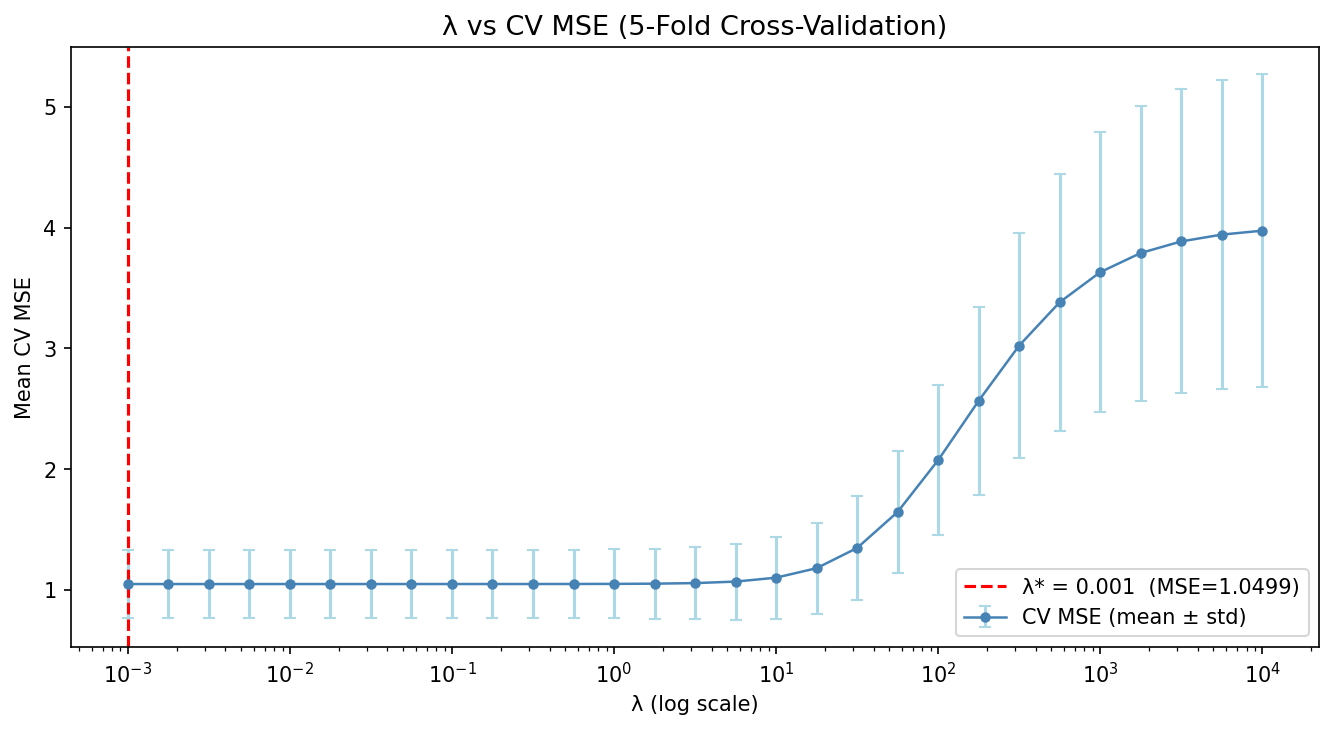
\includegraphics[width=0.82\textwidth]{assets/part1/lambda_cv_score.png}
    \caption{$\lambda$ vs CV-MSE (5-fold). Đường đỏ đứt là $\lambda^*$ tối ưu.
             Vùng $\lambda$ quá nhỏ: mô hình overfit (MSE cao trên validation);
             $\lambda$ quá lớn: underfit do shrinkage quá mạnh.}
    \label{fig:lambda_cv}
\end{figure}


